% !TeX root = ../sameplaper.tex
% !TeX spellcheck = en_US

\chapter{Lattices}
\setcounter{section}{0}


\section{Basics}
Lattices are the building blocks of lattice-based cryptography.
They find many applications in computer science and mathematics, including integer programming, diophantine approximation, cryptanalysis, the design of error-correcting codes for multi-antenna systems, and many more.
Currently, it is under prime focus among the cryptographic community due to its resistance towards attack by classical and quantum computers and some excellent properties that can be used to construct advanced cryptographic primitives, including fully homomorphic encryption, functional encryption, etc.

Lattices have been extensively used in cryptology in cryptanalysis (using lattice approximation algorithms to break cryptosystems) and in cryptography (using computationally hard lattice problems to design robust cryptographic schemes).
Furthermore, lattice-based encryption scheme enjoys solid security proofs based on worst-case hardness, relatively efficient implementations, and great simplicity.
Our primary focus here will be to discuss lattice primitives necessary to understand the practical aspects of lattice-based cryptography and homomorphic encryption and remain under this barrier.
For in-depth knowledge on lattices-based cryptography, exploration of survey paper \cite{peikert2016decade,nguyen2001two,micciancio2009lattice,peikert2016decade,regev2006lattice}, lecture notes \cite{MicciancioLN,regevlatticenotes,Vinodlatticenotes} and book \cite{MGbook} might be resourceful.

A lattice can be defined as the linear combinations with integer coefficients of the subgroup of any basis in $\mathbb{R}^n$.
More formally, it can be defined as
\begin{definition}
  Let $n\geq 1$ and let $\pmb{b}_1, \pmb{b}_2, \cdots, \pmb{b}_m$ be a basis of $\mathbb{R}^n$.
    The lattice with dimension $n$ and basis $\pmb{b}_1,\pmb{b}_2, \cdots, \pmb{b}_m$ is the set $\Lambda$ of all linear combinations of the basis vectors with integer coefficients:
    \begin{equation*}
        \Lambda(\pmb{b}_1,\cdots,\pmb{b}_m)=\mathbb{Z}\pmb{b}_1+\mathbb{Z}\pmb{b}_2+ \cdots + \mathbb{Z}\pmb{b}_m = \Big\{ \sum_{i=1}^{m} a_i\pmb{b}_i | a_1,a_2,\cdots,a_m \in \mathbb{Z} \Big\}
    \end{equation*}
\end{definition}
The basis vectors $\boldsymbol{b}_{1} ,\boldsymbol{b}_{2}, \cdots ,\boldsymbol{b}_{m}$ are said to be the generators of the lattice.
All bases have the same number of elements and are known as the $dimension$ of the lattice.
In this case, we have a lattice of $rank$ $m$ and $dimension$ $n$.
A lattice is said to be full rank when $n=m$.
In Figure \ref{fig:2ed_basis}, 2d-lattice generated by different basis vectors have been shown by Figure \ref{fig:1st_basis} and \ref{fig:2ed_basis} respectively.

The determinant of the lattice $\Lambda$ with basis $\pmb{b}_1, \pmb{b}_2, \cdots, \pmb{b}_n$ is defined as
\begin{equation*}
    det(\Lambda)=|det(\pmb{B})|
\end{equation*}

where $\pmb{B}$-- a $n\times n$ basis matrix with $\pmb{b}_i$ as its column.
Geometrically it corresponds to the inverse of the density of the lattice points in $\mathbb{R}^n$.
It is to be noted that the determinant of a lattice does not depend on the basis; another basis of the same lattice can be obtained by multiplying with an unimodular (determinant $\pm1$) matrix.


%https://cseweb.ucsd.edu/~daniele/papers/PostQuantum.pdf
%https://pure.tue.nl/ws/portalfiles/portal/47023806/719274-1.pdf
%https://cseweb.ucsd.edu/~daniele/papers/PostQuantum.pdf
%https://cseweb.ucsd.edu/classes/wi12/cse206A-a/lec1.pdf
%https://web.cs.ucla.edu/~nmanohar/nmanohar_files/UndergradThesis.pdf
When we study lattices, often we come across dual of a lattice, a dual of a lattice $\Lambda$ in $\mathbb{R}^n$ denoted by $\Lambda^{*}$ is defined as %the set of all vectors $\pmb{y} \in \mathbb{R}^n$ that satisfies
\begin{equation*}
    \Lambda^{*} =\{ \pmb{y} \in \mathbb{R}^n \ |\ <\pmb{x}, \pmb{y}> \ \in\ \mathbb{Z} \ \text{ for all vectors } \pmb{x} \in \Lambda \}
\end{equation*}
In general,
\begin{equation*}
    \Lambda^{*} =\{ \pmb{y} \in \text{span}(\Lambda) \ |\ <\pmb{x}, \pmb{y}> \ \in\ \mathbb{Z} \ \text{ for all vectors } \pmb{x} \in \Lambda \}
\end{equation*}

The lattice of integer points satisfies $(\mathbb{Z}^n)^* = \mathbb{Z}^n$ (and hence it is also addressed by self-dual).
Similarly, $(2\mathbb{Z}^n)^* =\frac{1}{2}\mathbb{Z}^n$.
It can be shown that for any basis $\pmb{B} \in \mathbb{R}^{n\times n}$, $\Lambda(\pmb{B})^{*} = \Lambda((\pmb{B}^{-1})^T)$.
From this it follows that $det(\Lambda^{*}) = \frac{1}{det(\Lambda)}$.


We often come across $q$-ary lattices in lattice cryptography and homomorphic encryption.
These are the lattices $\Lambda$ satisfying $q\mathbb{Z}^n \subseteq \Lambda \subseteq \mathbb{Z}^n$ for some (possibly prime) integer $q$.
This can also be understood as the lattice $\Lambda$ where the membership of a vector $\boldsymbol{x}$ in $\Lambda$ is determined by $\boldsymbol{x}$ mod $q$.
$q$-ary lattices are in one-to-one correspondence with linear codes in $\mathbb{Z}^n_q$.
In lattice cryptography, most constructions use $q$-ary lattices as their hard-on-average problem.
We can also say that any integer lattice $\Lambda \subseteq \mathbb{Z}^n$ is a $q$-ary lattice for some $q$, whenever $q$ is an integer multiple of the determinant $det(\Lambda)$.
However, in cryptographic applications, $q$ is usually kept much smaller than $det(\Lambda)$.

Given a matrix $\pmb{A} \in \mathbb{Z}^{n\times m}$ for parameters $q,m$ and $n$, we can define q-ary lattices as
\begin{align*}
    \Lambda_q(\pmb{A})         & = \{\pmb{y} \in \mathbb{Z}^m : \pmb{y = A^Ts} \text{ mod q for some } \pmb{s} \in \mathbb{Z}^n \} \\
    \Lambda^{\perp}_q(\pmb{A}) & = \{\pmb{y} \in \mathbb{Z}^m : \pmb{Ay = 0} \text{ mod }q \}
\end{align*}

In the definition above first $q$-ary lattice is generated by the rows of matrix $\pmb{A}$. In contrast, the second $q$-ary lattice contains all orthogonal vectors with respect to rows of $\pmb{A}$ modulo $q$.
It is clear from the dual definition above that these two lattices are dual to each other up to normalization, namely,
$\Lambda^{\perp}_q(\pmb{A}) = q \cdot \Lambda_q(\pmb{A})^{*}$ and
$\Lambda_q(\pmb{A}) = q \cdot \Lambda^{\perp}_q(\pmb{A})^{*}$.
%https://cseweb.ucsd.edu/~daniele/papers/PostQuantum.pdf


Fundamental parallelepiped generated by the basis matrix $\pmb{B}$ is defined as
\begin{align*}
    P(\pmb{B}) & =\{\pmb{Bx} \ | \ \pmb{x} \in [0,1)^n\}
\end{align*}
%https://ocw.mit.edu/courses/18-409-topics-in-theoretical-computer-science-an-algorithmists-toolkit-fall-2009/a5351bd811ac52366dec759f2c6b2fac_MIT18_409F09_scribe18.pdf

%http://www.cs.umd.edu/~gasarch/BLOGPAPERS/RegevLWEtalk.pdf
%https://eprint.iacr.org/2012/533.pdf






%--------------lattice figure-----------------------
\begin{figure}[h!]
    \centering
    \begin{subfigure}[t]{0.48\textwidth}
        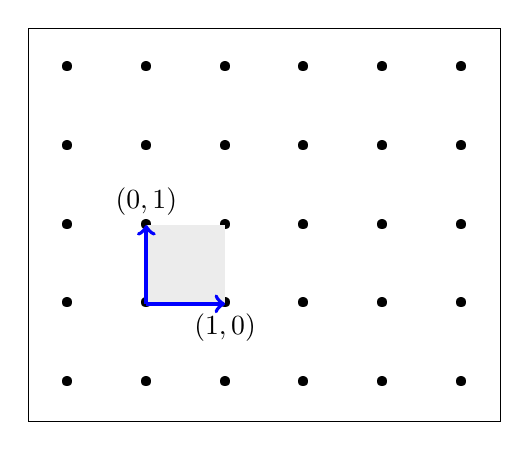
\begin{tikzpicture}
            \draw[color=black] (-3.5,3.5) -- (2.5,3.5) -- (2.5,-1.5) -- (-3.5,-1.5) --  (-3.5,3.5);
            \foreach \Point in {(-3,3), (-3,2), (-3,1), (-3,0), (-3,-1),
                    (-2,3), (-2,2), (-2,1), (-2,0), (-2,-1),
                    (-1,3), (-1,2), (-1,1), (-1,0), (-1,-1),
                    (0,3),  (0,2),  (0,1),  (0,0),  (0,-1),
                    (1,3),  (1,2),  (1,1),  (1,0),  (1,-1),
                    (2,3),  (2,2),  (2,1),  (2,0),  (2,-1)}{
                    \node at \Point {\textbullet};
                }
            \fill [color=gray!15] (-2,0) rectangle (-1,1);
            \draw[->, thick, line width=.5mm,  blue] (-2,0)--(-2,1); % l'axe des abscisses
            \draw[->, thick, line width=.5mm,  blue] (-2,0)--(-1,0); % l'axe des ordonnées
            \node at (-2,1.3) {$(0,1)$};
            \node at (-1,-.3) {$(1,0)$};

        \end{tikzpicture}
        \caption{Basis in 2d lattice}
        \label{fig:1st_basis}
    \end{subfigure}\quad%
    \begin{subfigure}[t]{0.48\textwidth}
        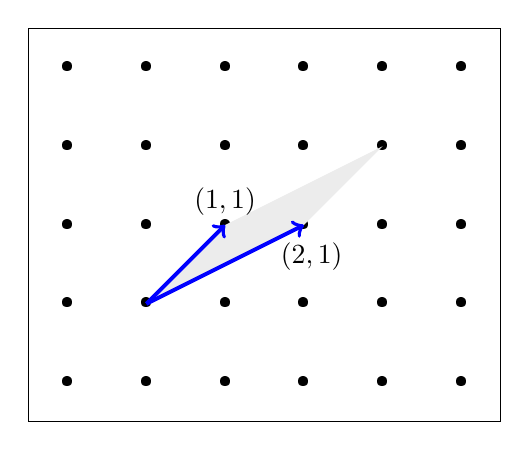
\begin{tikzpicture}
            \draw[color=black] (4.5,3.5) -- (10.5,3.5) -- (10.5,-1.5) -- (4.5,-1.5) --  (4.5,3.5);
            \foreach \Point in {(5,3), (5,2), (5,1), (5,0), (5,-1),
                    (6,3), (6,2), (6,1), (6,0), (6,-1),
                    (7,3), (7,2), (7,1), (7,0), (7,-1),
                    (8,3), (8,2), (8,1), (8,0), (8,-1),
                    (9,3), (9,2), (9,1), (9,0), (9,-1),
                    (10,3), (10,2), (10,1), (10,0), (10,-1)}{
                    \node at \Point {\textbullet};
                }
            \fill[color=gray!15] (6,0) -- (8,1) -- (9,2) -- (7,1) --  (6,0);
            \draw[->, thick, line width=.5mm,  blue] (6,0)--(7,1); % l'axe des abscisses
            \draw[->, thick, line width=.5mm,  blue] (6,0)--(8,1); % l'axe des ordonnées
            \node at (7,1.3) {$(1,1)$};
            \node at (8.1,.6) {$(2,1)$};

        \end{tikzpicture}
        \caption{Another basis in the same lattice}
        \label{fig:2ed_basis}
    \end{subfigure}
    \caption{Figure \ref{fig:1st_basis} shows the lattice generated by $(1,0)$ and $(0,1)$ in $\mathbb{Z}^2$, it is the lattice of all integers points in $\mathbb{Z}^2$.
        However, this is not unique and can also be generated as shown in the figure\ref{fig:2ed_basis} with $(1,1)$ and $(2,1)$.
        Similarly, Yet another example of basis in $\mathbb{Z}^2$ can be generated by $(2021, 1)$ and $(2022, 1)$.
        However, it is to be noted that $(1, 1)$ and $(2,0)$ are not a basis of $\mathbb{Z}^2$; this is because it only generates the lattice of all integer points whose coordinates sum to an even number.
        All examples mentioned so far are full-rank lattices.
        An example of a lattice that is not full is $\Lambda((2, 1))$. It is of rank one and dimension 2.
        A one-dimensional lattice of full-rank is the lattice $\mathbb{Z}= \Lambda((1))$.}
    \label{fig:Basis_of_2d_lattice}
\end{figure}
%-----------Figure ends here---------------


In Figure \ref{fig:Basis_of_2d_lattice}, fundamental parallelepiped $P(\pmb{B})$ is shown by the gray-shaded region.
Note that $P(\pmb{B})$ not only depends on the lattice but also on the choice of the basis $\pmb{B}$.
A basis is termed a `good' or a `bad' based on the type of parallelepiped it forms.
A good basis is the one that forms a square-like parallelepiped, while a `bad' basis is the one that creates a very thin parallelepiped as shown by Figure \ref{fig:1st_basis} and \ref{fig:2ed_basis} respectively.

%https://eprint.iacr.org/2012/533.pdf
%https://web.cs.ucla.edu/~nmanohar/nmanohar_files/UndergradThesis.pdf
In lattice, there are several hard problems.
The conjectured intractability of such problems is central to constructing secure lattice-based cryptosystems.
The most common ones include the following:

\begin{definition}
    Shortest Vector Problem (SVP): Given a lattice basis, the problem is to find the shortest non-zero vector present in the lattice.
    Mathematically, given a lattice basis $\pmb{B}\in \mathbb{Z}^{m \times n}$, find a nonzero lattice vector $\pmb{Bx}$, $\pmb{x}\neq \pmb{0}, \pmb{x} \in \mathbb{Z}^n$, such that $||\pmb{Bx}|| \leq ||\pmb{By}||$, $\forall \pmb{y} \in \mathbb{Z}^n$.%and $\pmb{y} \neq \pmb{0}$.
\end{definition}
In practice, the length of the shortest non-zero vector present in a lattice $\Lambda$ is denoted by $\lambda_1(\Lambda)$ and $i^{th}$ successive minimum by $\lambda_i(\Lambda)$.
The $i$-th successive minimum $\lambda_i(\Lambda)$ is the radius $r$ of the smallest $n$-dimensional (Euclidean) ball that contains $i$ linearly independent vectors in $\Lambda$.
Mathematically,
\begin{equation*}
    \lambda_i(\Lambda) = min\{r > 0 | dim(span(\Lambda \cap rU)) \geq i\}
\end{equation*}
where U is the unit ball in the Euclidean norm \cite{laarhoven2012solving}.

%https://eprint.iacr.org/2016/146.pdf
An $n$-dimensional Euclidean ball of radius $R$ denoted by $Ball_n(R)$ has a volume of
\begin{equation*}
    V_n(R) = R^n \frac{\pi^{n/2}}{\Gamma(n/2+1)}
\end{equation*}
where Stirling's approximation yields $\Gamma(n/2+1) \approx \sqrt{\pi n}(n/2)^{n/2}e^{-n/2}$ and $V_n(1)^{-1/n} \approx \sqrt{n/(2\pi e)} \approx \sqrt{n/17}$

The Gaussian Heuristic approximates the number of lattice points in a continuous (usually convex and symmetric) set $S\subset R^n$.
To be more precise, it says that for a given set $S$ and a lattice $\Lambda$, we get $|S\cap \Lambda| \approx vol(S)/det(\Lambda)$.

Considering $S$ as the origin-centered ball of radius $R$, the number of lattice points is approximately $V_n(R)/vol(\Lambda)$, Thus the length of shortest vector $\lambda_1$ in a ball of radius $R$ is
\begin{equation*}
    \lambda_1(\Lambda) \approx det(\Lambda)^{1/n}/ V_n(1)^{1/n}= \frac{(\Gamma(n/2+1)det(\Lambda))^{1/n}}{\sqrt{\pi}}
\end{equation*}
%This is called the Gaussian heuristic of a lattice and is denoted by $GH(\mathcal{L})=det(\mathcal{L})^{1/n}/ V_n(1)^{1/n}$

%Gaussian heuristic suggests that the shortest vector in a lattice $L$ of rank $m$ has Euclidean norm about $\frac{1}{\sqrt{\pi}} \Gamma(1+\frac{m}{2})^{1/m} Vol(\mathcal{L})^{1/m}$,
which is approximately $\sqrt{\frac{n}{2\pi e}} Vol(\Lambda)^{1/n}$.
In a $q$-ary lattice $\Lambda$ (of rank $m$), this is $\sqrt{\frac{m}{2\pi e}}q^{(m-n)/m}$.
A $q$-ary lattices contain known vectors of Euclidean length equal to $q$.
Hence, an estimate of the Euclidean length of known short vectors is

\begin{equation}
    \lambda_1(\Lambda) \approx min \Big\{q,\sqrt{\frac{m}{2\pi e}} q^{\frac{m-n}{m}} \Big\}
\end{equation}

%\lambda_2(L') \approx

\begin{comment}


In contrast, the vector $\pmb{e}$ has Euclidean length around $\sqrt{m}\delta$
on average and so the vector $(\frac{e}{M})$ has length approximately $\sqrt{2m}\sigma$ when $M = \sqrt{m}\sigma$.
In our experiments we take $M = 1$ and so assume that $\lambda_1(L') \approx \sqrt{m}\sigma$.
Hence the gap is
\begin{equation}
    \gamma(m) = \frac{\lambda_2(L')}{\lambda_1(L')} \approx \frac{min\{q,\frac{1}{\sqrt{\pi}} \Gamma(1+\frac{m}{2})^{\frac{1}{m}}q^{\frac{m-n}{m}}}{\sqrt{m}\sigma} \approx \frac{min\{q, \sqrt{\frac{m}{2\pi e}}q^{\frac{m-n}{m}}\}}{\sqrt{m}\sigma}
\end{equation}
For a successful attack we want this gap to be large, so we will need
\begin{equation}
    \sigma << q^{\frac{m-n}{m}} < \frac{q}{\sqrt{m}}
\end{equation}

To determine whether an LWE instance can be solved using the embedding technique and a lattice reduction algorithm with a given (root) Hermite factor $\delta$, one can choose a suitable subdimension $m$ and verify that the corresponding gap satisfies the condition $\gamma = \gamma(m) > c\delta^m$ for a suitable value $c$.
Since the constant $c$ is unknown, we can maximize $min{q, q^{\frac{m-n}{m}}}/\delta^m$ for fixed $n$, $q$, $\delta$ to get the ``optimal” sub-dimension (which maximizes the success probability of the algorithm) to be
\begin{equation}
    m = \sqrt{\frac{n\log{(q)}}{\log{(\delta)}}}
\end{equation}
where $\delta$ is the Hermite factor of the lattice basis reduction algorithm used.


It is to be noted that ISIS problem can be attacked by reducing it to CVP problem.
Considering a lattice $\mathcal{L}'= \Lambda^\perp_q(A^T)=\{ y \in \mathbb{Z}^m : A^Ty \equiv 0 (mod q)\}$, finds any vector (not necessarily short) $w \in Z^m$ such that $A^Tw \equiv v (mod q)$, then solves CVP for $(L', w)$ to find some $y$ close to $w$ and so returns $w-y$ as the ISIS solution.

We sketch the details of solving LWE (in the case of short secrets) by reducing
to ISIS and then solving by CVP.
Given $(A, b)$ we define $A' = (A|I_m)$ to get an ISIS instance $(A',b)$.
Choose any vector $w \in Z^{n+m}$ such that $A'w \equiv b$ (mod $q$).
Then the lattice $L' = \Lambda^{\perp}_q(A') = \{y \in Z^{n+m} : A'y \equiv 0 (\ mod\ q)\}$ is seen to have rank $m'=n+m$ and (assuming the rank of $A'$ is $n$) determinant $q^m = q^{m'-n}$ (the determinant condition can be seen by considering the index of the subgroup $qZ^{n+m}$ in the additive group $L'$).
The condition for success in the algorithm is $\sigma << q^{m/(n+m)}$.
Writing $m' = n+m$ this is $q^{(m'-n)/m'}$, which is the same as the LWE condition above
\end{comment}




\begin{definition}
    Closest Vector Problem (CVP): Given a lattice basis and a target vector (not necessarily from the lattice), the problem is to find a lattice vector in the given lattice closest to the target vector.
    Mathematically, given a lattice basis $\pmb{B}\in \mathbb{Z}^{m \times n}$ and a target vector $\pmb{t} \in \mathbb{Z}^m$, the problem is to find a lattice vector $\pmb{v}=\pmb{Bx}$ for some $\pmb{x} \in \mathbb{Z}^n$, such that $||\pmb{v}-\pmb{t}|| \leq ||\pmb{By}-\pmb{t}||$ for all $\pmb{y} \in \mathbb{Z}^n$
\end{definition}

\begin{definition}
    Shortest Independent Vectors Problem (SIVP): Given a lattice basis, the problem is to find $n$ (dimension of the lattice) linearly independent lattice vectors with minimum length (Euclidean norm).
    Alternatively, it asks for a new basis that yields the same lattice but with a minimum length of the longest vector.
    Mathematically, given a lattice basis $\pmb{B}\in \mathbb{Z}^{m \times n}$, find lattice vectors $\pmb{Bx}_1, \cdots, \pmb{Bx}_n \in \mathbb{Z}^m$, $\pmb{x}_1,\cdots,\pmb{x}_n \in \mathbb{Z}^n$ that are linearly independent and $||\pmb{Bx}_i|| \leq \lambda_n(\Lambda (\pmb{B})$ for $1 \leq i \leq n$.
\end{definition}

In literature, besides the above problems, the Shortest Integer Solution (SIS) problem finds many applications, including its use in solving LWE.
The SIS problem is defined as

\begin{definition}Short Integer Solution (SIS) problem:
    Given a $q$-ary lattice, the problem is to find an orthogonal vector with a restricted norm.
    Formally, given a lattice basis generated by integer matrix $\pmb{A}^{m \times n}$ (where typically $m$ is much bigger than $n$) and an integer modulus $q$ the problem is to find a vector $\pmb{y}$, $0<||\pmb{y}||\leq \beta$ if it exists, such that $\pmb{A}^T\pmb{y} \equiv 0 \ ( \text{mod} \ q)$.
    %$\pmb{y} \in \pmb{B}$ a set of vectors that are “short” in some sense (e.g., $\pmb{B} = \{-1,0,1\}^m$), with $||\pmb{y}||\leq \beta$ if it exists, such that $\pmb{A}^T\pmb{y} \equiv 0 \ ( \text{mod} \ q)$.

    A variant of this problem is known as the inhomogeneous SIS problem (ISIS), where given $\pmb{A}$ and $\pmb{v}$ find $\pmb{y}$,
    % \in \pmb{B}$,
    $0<||\pmb{y}||\leq \beta$ if it exists, such that $\pmb{A}^T\pmb{y} \equiv \pmb{v} \ ( \text{mod} \ q)$.
\end{definition}

A solution to the ISIS problem gives a value for the error $\pmb{e}$ and can be used to solve the LWE problem.
However, we need to rephrase the LWE problem into the ISIS problem.
There are two ways to rephrase the LWE problem into the ISIS problem in the literature mentioned in \cite{bai2014lattice} and \cite{micciancio2011pseudorandom}, respectively.

Bai and Galbraith’s \cite{bai2014lattice} way of rephrasing the LWE problem into an ISIS problem goes as follows: given $(\pmb{A}, \pmb{b} \equiv \pmb{As} + \pmb{e}$ (mod $q$)) one can form the ISIS instance as
\begin{equation*}
    (\pmb{A} | \pmb{I}_m)
    \begin{pmatrix}
        \pmb{s} \\
        \pmb{e}
    \end{pmatrix}
    \equiv b \ (\text{mod} \ q)
\end{equation*}
where $I_m$ is the $m \times m$ identity matrix.

Micciancio and Mol present an alternative way of transforming the LWE problem into an ISIS problem in \cite{micciancio2011pseudorandom}.
The technique is to construct a matrix $\pmb{G} \in \mathbb{Z}^{(m-n)\times m}_q$ such that $\pmb{GA} \equiv 0$ (mod $q$).
Thus the LWE problem ($\pmb{A}$, $\pmb{b}$) gets transformed into the ISIS instance as ($\pmb{G},\pmb{Gb}\equiv \pmb{Ge}$ (mod $q$)).
More detail about the same can be obtained in lemma 9 and 10 of \cite{micciancio2011pseudorandom}.


It is to be noted that both approaches are equivalent when the secret vector $\pmb{s}$ is chosen from the error distribution.
However, when the secret vector $\pmb{s}$ is chosen from a ``small" distribution, the earlier approach is better than the latter one.
This is because the reduction eliminates the vector s. Thus the advantage of the secret $\pmb{s}$ being ``small'' compared with $\pmb{e}$ no longer can be used.


%Remark: we usually consider Euclidean norm however any norm it should work.
%\textbf{Geometric Series Assumption}

An approximate variant of the above problems is often considered in lattice cryptography.
Approximate variants are denoted by an additional parameter $\gamma$ as a subscript, usually indicating the approximation factor.
For instance, in $SVP_\gamma$ the goal is to find a vector whose norm is at most $\gamma$ times that of the shortest nonzero vector present in the lattice.
It is to be noted that lattice problems can be defined for any norm, but in practice, Euclidean norm $||\pmb{x}||=\sqrt{\sum_i x^2_i}$ is the most common one \cite{peikert2008limits}.

\section{Lattice reduction}
Lattice reduction algorithms are used to convert a bad basis into a good basis \cite{laarhoven2012solving}.
Working on a good basis, viz., finding a short vector, is comparatively easier than working on a bad basis.
Thus bad basis is converted into a good basis for practical lattice attacks and is done by lattice reduction algorithms.
Alternatively, lattice reduction plays a central step in breaking hard lattice problems.
Hence without reviewing lattice reduction algorithms explaining lattice attacks on hard lattice problems will be incomplete.
Thus in the following few pages, we will briefly discuss the different lattice reduction algorithms from the literature.


Using lattice reduction viz., BKZ, Schnorr in \cite{schnorr2003lattice} introduced the geometric series assumption (GSA) to find the Gram-Schmidt length ($||\pmb{b}_i^*||$) of BKZ-reduced basis.
It says that the BKZ-reduced basis decay geometrically with quotient $r$ for $i = 1,\cdots,n$, viz.,
\begin{equation*}
    ||\pmb{b}_i^*||^2/||\pmb{b}_1||^2=r^{i-1} \hspace{2em} for \ some \ r \in [3/4,1)
\end{equation*}
$r$ here represents the GSA constant.


%--------------start lattice relation figure-----------------------
\begin{figure}[h!]
    \centering
    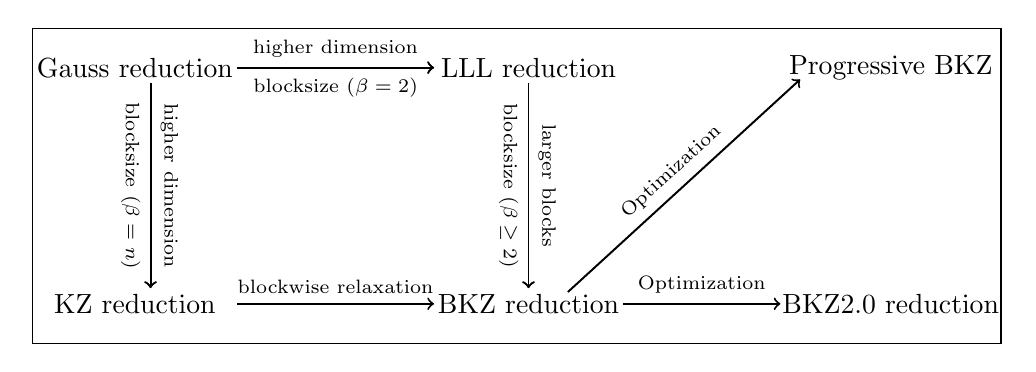
\begin{tikzpicture}
        %box drawing
        \draw[color=black] (-6.3,.5) -- (6,.5) -- (6,-3.5) -- (-6.3,-3.5) --  (-6.3,.5);
        % horizental
        \draw[->, line width=.25mm,  black] (-3.7,0)--(-1.2,0) node[midway,above,font=\scriptsize] {higher dimension};
        \draw[->, line width=.25mm,  black] (-3.7,0)--(-1.2,0)  node[midway,below,font=\scriptsize] {blocksize ($\beta=2)$};

        %Curved
        \draw[->, line width=.25mm,  black] (.5,-2.85)--(3.45,-.15) node[midway,above,font=\scriptsize,sloped] {Optimization};


        \draw[->, line width=.25mm,  black] (-3.7,-3)--(-1.2,-3) node[midway,above,font=\scriptsize] {blockwise relaxation};
        \draw[->, line width=.25mm,  black] (1.2,-3)--(3.2,-3) node[midway,above,font=\scriptsize] {Optimization};

        % Vertical
        \draw[->, line width=.25mm,  black] (-4.8,-.2)--(-4.8,-2.8) node[midway,above,font=\scriptsize,sloped] {higher dimension};
        \draw[->, line width=.25mm,  black] (-4.8,-.2)--(-4.8,-2.8) node[midway,below,font=\scriptsize,sloped] {blocksize ($\beta=n$)};

        \draw[->, line width=.25mm,  black] (0,-.2)--(0,-2.8) node[midway,above,font=\scriptsize,sloped] {larger blocks};
        \draw[->, line width=.25mm,  black] (0,-.2)--(0,-2.8) node[midway,below,font=\scriptsize,sloped] {blocksize ($\beta \geq 2)$};


        \node at (-5,0) {Gauss reduction};
        \node at (0,0) {LLL reduction};
        \node at (-5,-3) {KZ reduction};
        \node at (0,-3) {BKZ reduction};
        \node at (4.6,-3) {BKZ2.0 reduction};
        \node at (4.6,0) {Progressive BKZ};
    \end{tikzpicture}
    \caption{Overview of the basis reduction algorithms.} %(Picture taken from \cite{laarhoven2012solving})}
    \label{fig:lattice_relations}
\end{figure}
%--------------end lattice relation figure-----------------------

Lattice reduction algorithms can be viewed as a hierarchy of BKZ algorithms based on the block parameter $k$ used for the lattice reduction as shown in Figure \ref{fig:lattice_relations}.
When $k=2$, the BKZ algorithms run in polynomial time, but the reduced basis will only be LLL-reduced-- producing short vectors within exponential factors of a short vector.
When $k=n$, the reduced lattice is KZ (Korkine-Zolotarev) reduced or HKZ (Hermite-Korkine-Zolotarev) reduced -- this is in some way optimally reduced but takes exponential run time.
Thus usually, lattice reduction is performed based on intermediate block size, which is decided based on the required root Hermite factor (discussed below).
When optimization is used to optimize the BKZ algorithm's run time, it gives rise to BKZ2.0.
Further optimization to the BKZ is known as the Progressive BKZ, as shown in Figure \ref{fig:lattice_relations}.

Gama and Nguyen \cite{gama2008predicting} provided a heuristic to estimate the shortest vector produced by lattice reduction algorithms.
Suppose a lattice reduction algorithm is fed with a basis of a lattice $\Lambda$ of dimension $n$, then the algorithm outputs a list of vectors $\pmb{b}_1,\pmb{b}_2,\cdots,\pmb{b}_n$.
The shortest vector produced by the lattice reduction algorithm can be approximated using the root Hermite factor, denoted by $\delta_0$, as defined in \cite{gama2008predicting} as

% Hermite factor is used to determine the quality of basis produced by a lattice reduction algorithm and is usually denoted by $\delta_0$. A Hermite factor is defined as the shortest non-zero vector $\textbf{b}_0$ produced by the lattice reduction algorithm and is represented as
\begin{equation}
    ||\pmb{b}_0||=\delta^n_0 \cdot \text{vol}(\Lambda)^{1/n}
    \label{eq:first_min}
\end{equation}
%https://eprint.iacr.org/2013/839.pdf
Considering $m$ samples in a $q$-ary lattice the expression \ref{eq:first_min} above simplifies to
\begin{equation*}
    ||\pmb{b}_0|| \approx \delta^m_0 \cdot \text{vol}(\Lambda)^{n/m}
\end{equation*}
with high probability, where $n$ is the LWE dimension and $m$ is the number of samples under consideration.
The minimum of the expression above is attained for $m=\sqrt{\frac{n\log{q}}{\log \delta_0}}$ \cite{Micciancio2009}.

LLL algorithm produces $\delta = 1.021$.
Gama and Nguyen in \cite{gama2008predicting} argued that $\delta = 1.01$ is about the limit of practical algorithms (i.e., variants of BKZ using extreme pruning and large block size).
Chen and Nguyen in \cite{chen2011bkz} extended this analysis to algorithms with greater running time.
Their heuristic argument is that a Hermite factor corresponding to $\delta = 1.006$ might be reachable with an algorithm performing around $2^{110}$ operations.

Gama and Nguyen in \cite{gama2008predicting} focus on the unique-SVP problem.
One seeks a short vector in a lattice $\Lambda$ when one knows that there is a significant gap $\gamma = \lambda_2(\Lambda)/\lambda_1(\Lambda)$, where $\lambda_i(\Lambda)$ denotes the $i$-th successive minima of the lattice.
The unique SVP problem arises when solving CVP using the embedding technique.
The standard theoretical result is that if one uses a lattice reduction algorithm with Hermite factor $\delta$, the algorithm outputs the shortest vector if the lattice gap satisfies $\gamma > \delta^{2m}$.
However, Gama and Nguyen observe that practical algorithms will succeed as long as $\gamma > c\delta^m$ for some small constant $c$ (they provided values of $c = 0.26$ and $c = 0.45$ for different families of lattices).
Later, Luzzi, Stehl\'e, and Ling \cite{luzzi2013decoding} provided some theoretical justification claiming that the unique-SVP problem is easier to solve when the gap is significant.

Below we have briefly discussed different lattice reduction algorithms available in the literature with their run time and available implementations.




\subsection{Gauss Algorithm}
Gauss algorithm \cite{bremner2011lattice} (sometimes also attributed to Lagrange \cite{de1773recherches}) finds an optimally reduced basis in a two-dimensional lattice.
The optimally reduced basis $\{\pmb{b}_1,\pmb{b}_2\}$ in a $2$-dimensional lattice $\Lambda$ are such that $||\pmb{b}_1||=\lambda_1(\Lambda)$ and $||\pmb{b}_2||=\lambda_2(\Lambda)$.

%In this algorithm, we assume that at any point, the Gram-Schmidt coefficient µ2,1 = (b2 ·b1)/kb1k two is known and up to date with respect to the current vectors b1 and b2. For simplicity and to focus on the high-level description rather than the low-level details, in the algorithms discussed in this section we will omit details on updating the GSO-vectors b∗i and the coefficients µi, j.

The algorithm works as follows: in each iteration, the algorithm checks $||\pmb{b}_1|| \geq ||\pmb{b}_2||$.
If the condition evaluates to be true, then it swaps the vectors and subtract the shorter vector $\pmb{b}_1$ multiplied with integral multiple of $(\lfloor\mu_{2,1}\rceil = \lfloor \frac{(\pmb{b}_1 \cdot \pmb{b}_2)}{||\pmb{b}_1||^2}\rceil)$ from the longer vector $\pmb{b}_2$ to obtain a shorter vector $\pmb{b}_2 \leftarrow \pmb{b}_2 - \lfloor \mu_{2,1}\rceil\pmb{b}_1$ then it swaps the vectors $\pmb{b}_1$ and $\pmb{b}_2$.
The algorithm stops when the condition $||\pmb{b}_1|| \geq ||\pmb{b}_2||$ fails.
The algorithm upon completion produces $|\mu_{2,1}| \leq \frac{1}{2}$

The algorithm runs in poly($\log{||\pmb{B}||}$) time i.e.
in time polynomial in the size of the input basis $\pmb{B}$.






\subsection{LLL Algorithm}
LLL algorithm acronym of its designers name Lenstra-Lenstra-Lov\'{a}sz \cite{lenstra1982factoring} is the generalization of Gauss Algorithm\cite{bremner2011lattice} presented above to the higher dimension.
Extending the Gauss algorithm to the higher dimension may seem easy, but it's not.
This is due to the size-reduction and the swapping step; there are too many basis vectors to choose from, and one needs a procedure to make this choice.
It is finally achieved by imposing the following two conditions:
\begin{enumerate}
    \item $|\mu_{i,j}|\leq \frac{1}{2}$  \hspace{11.2em} for $0 \leq j < i \leq n-1$
    \item $||\pmb{v}_i^* + \mu_{i,i-1}\pmb{v}_{i-1}^*||^2 \geq \alpha ||\pmb{v}_{i-1}^*||^2$ \hspace{1.8em} for $2\leq i \leq n$
\end{enumerate}

%In two dimensional lattice, the lattice vectors $\{\pmb{v}_1,\pmb{v}_2\}$ is minimized by repeatedly performing swapping operation based on $||\pmb{v}_1|| \leq ||\pmb{v}_2||$ after performing $\pmb{v}_2=\pmb{v}_2-\lceil \frac{\pmb{v}_2 \cdot \pmb{v}_1}{\pmb{v}_1 \cdot \pmb{v}_1} \rfloor \pmb{v}_1$ until no further change can be made.
The minimal basis obtained by performing the above operations satisfies the inequality $ \mu_{2,1}=\frac{\pmb{v}_2 \cdot \pmb{v}_1}{\pmb{v}_1 \cdot \pmb{v}_1}\leq \frac{1}{2}$.



The first condition is known as Lov\'asz condition, and the second condition is known as the exchange condition.
Here $\alpha$ ($\frac{1}{4}<\alpha<1 $) represents the reduction parameter and $\pmb{v}^*_1,\pmb{v}^*_2,\cdots,\pmb{v}^*_n$ represents the orthogonal vector obtained using Gram-Schmid Orthogonalization \cite{lang2012introduction}.
As $\pmb{v}^*_1,\pmb{v}^*_2,\cdots,\pmb{v}^*_n$ are orthogonal to each other, exchange condition also evaluates to
\begin{enumerate}
    \item[$2'.$] $||\pmb{v}_i^*||^2 \geq (\alpha-\mu_{i,i-1}^2) ||\pmb{v}_{i-1}^*||^2$ \hspace{1.8em} for $2\leq i \leq n$
\end{enumerate}

In brief, the LLL algorithm works by size reduction of basis vectors pairwise followed by Lov\'asz condition checking to confirm if the Lov\'asz condition still holds; if it does not, then it performs the vector swap operation between the current vector to that of the previous vector.
More detail about the LLL algorithm can be obtained in section 4.3 of \cite{bremner2011lattice}.

There are many variants of the original LLL algorithm available in the literature.
One of the well-known variants is the LLL by deep
insertions, proposed by Schnorr and Euchner \cite{schnorr1994lattice}.
The idea is to rather than swapping two neighboring basis vectors $\pmb{b}_i$ and $\pmb{b}_{i-1}$; this algorithm inserts $\pmb{b}_i$ somewhere in the basis, at some position $j<i$.
In short, this further generalizes the original LLL algorithm since taking $ j=i-1 $ for each swap leads to the original LLL algorithm.
The position of insertion of vector $\pmb{b}_i$ is decided based on the smallest index $j$ that gains a factor of at least $\delta$, same as that of proof of the LLL algorithm.
This slight modification in the original LLL leads to shorter vectors with a longer run time.

LLL algorithm runs in polynomial time \cite{bremner2011lattice}, given a rank $m$ integer lattice with basis vectors of Euclidean norm less than $\pmb{B}$ in an $n$-dimensional space, the LLL algorithm outputs a reduced basis in time $O(m^3n \log{\pmb{B}}\cdot M(m\log{\pmb{B}}))$ bit operations, where $M(k)$ represents the multiplication time of $k$-bit integers.
Presence of $m$ and/or $\log{\pmb{B}}$ makes the worst-case time complexity of the original LLL algorithm relatively high for applications where they are significantly large.
To reduce computational complexity, Nguyen and Stehl\'e proposed a variant of the LLL algorithm in \cite{nguyen2009lll}, that has a run time of $O(m^2n(m+\log{\pmb{B}}) \log{\pmb{B}}\cdot M(m))$.
In \cite{chen2011bkz}, Chen and Nguyen performed modification to the fplll\cite{cade2008fplll}, using \cite{novocin2011lll} and reported a heuristic run time of the LLL algorithm as $O(n^3\log^2\pmb{B})$.

In the original LLL paper \cite{lenstra1982factoring}, it has been reported that theoretically, LLL achieves a Hermite factor of $(\frac{4}{3})^{\frac{(n-1)}{4}}=1.07456^{(n-1)}$, however in practice it behaves much better.
In \cite{gama2008predicting}, it has been reported that LLL achieves a root-Hermite factor of $\delta_0= 1.0219^n$ for large dimension $n$.
The constant $1.0219$ that appeared in the above result has been investigated in \cite{vallee2009probabilistic} and tried to provide mathematical backing, but they reported that the problem is still too hard to explain.
In short, there are still several open problems in this area.
%https://eprint.iacr.org/2012/533.pdf

Implementation of the LLL algorithm can be obtained in many software packages, few of them includes fpLLL\cite{fplll}, Magma\cite{MR1484478}, Mathematica\cite{Mathematica}, NTL\cite{Shoup_LLL}, PARI/GP\cite{PARI2}, SageMath\cite{sagemath} etc.





\subsection{BKZ Algorithm} In $2$-dimensional lattice, the Gauss algorithm finds an optimal base later generalized by the LLL to the higher dimensional lattice using block size $\beta=2$.
It is known that when the bases are Korkine-Zolotarev (KZ) reduced \cite{korkine1873formes} or Hermite-Korkine-Zolotarev (HKZ) reduced (Gram-Schmidt vectors of basis $\{\pmb{b}_1,\cdots,\pmb{b}_n\}$ satisfy $||\pmb{b}_i^*||=\lambda_1(\pi_i(\Lambda))$ for all $i$) it produces an optimally reduced basis, but finding such bases is known to be hard in higher dimensions.
It is at least as hard as finding the shortest vector in $n$-dimensional lattice since the shortest basis vector is the shortest vector of the lattice.
Thus as the dimension increases, the algorithm and hence the notion of reduction becomes impractical.
Alternatively, this algorithm terminates in a reasonable amount of time when the dimension $n$ is sufficiently small.
Hence, if we want to find nice bases for an arbitrary dimensional lattice, we need a different method.

Block Korkine-Zolotarev algorithm \cite{schnorr1994lattice} also known as the BKZ, was proposed in this direction that works by forming a local lattice block of small size represented by blocksize $\beta \geq 2$ (usually block size $\beta$ is very small compared to the dimension $n$).
BKZ, for each block, calls a subroutine that solves the exact SVP problem.
Typically, SVP can be solved by three different techniques, viz.,
enumeration, computing the Voronoi cell of the lattice, or by sieving.
The cost of solving SVP, using different techniques, takes different time and memory as presented in the table \ref{tab:BKZ_SVP_cost}.
When SVP is solved using enumeration, BKZ calls the enumeration subroutine \cite{schnorr1994lattice,kannan1983improved,fincke1985improved,pohst1981computation} many times, which looks for the nearly-shortest vector in the projected lattices of dimension $\leq \beta$.
The higher the value of $\beta$, the more reduced the basis will be, and the cost of reduction will also be higher.
\begin{table}[h!]
    \centering
    \begin{center}
        \begin{tabular}{|c|c|c|c|}%|p{3.7cm}|p{2.5cm}|p{2.5cm}|p{2.5cm}|}
            \hline
            Techniques                           & Time              & Space             & Operation Mode \\
            \hline
            Enumeration [FiPo’83,Kan’83,HaSt’07] & $n^{n/(2e)+o(n)}$ & $Poly(n)$         & Deterministic  \\
            \hline
            Sieving [AjKuSi’01,PuSt’09]          & $2^{2.247n+o(n)}$ & $2^{1.325n+o(n)}$ & Probabilistic  \\
            \hline
            Heuristic Sieving [MiVo’10,BDGL’16]  & $2^{0.292n+o(n)}$ & $2^{0.292n+o(n)}$ & Heuristic      \\
            \hline
            Voronoi cell [MiVo’10]               & $2^{2n+o(n)}$     & $2^{n+o(n)}$      & Deterministic  \\
            \hline
            Gaussians [ADRS’16]                  & $2^{n+o(n)}$      & $2^{n+o(n)}$      & Probabilistic  \\
            \hline
        \end{tabular}
    \end{center}
    \caption{Runtime of different SVP computation techniques available in the literature}
    %https://www.issac-conference.org/2017/assets/tutorial_slides/Stehle.pdf   page 13
    \label{tab:BKZ_SVP_cost}
\end{table}


Typically BKZ algorithm works as follows: for an input basis $\pmb{B}_{[1,n]} = (\pmb{b}_1, \cdots, \pmb{b}_n)$ of lattice $\Lambda$, it starts by reducing the basis $\pmb{B}_{[1,n]}$ into the LLL, then it calls the SVP oracle that reduces and enumerates each local block $\pmb{B}_{[j, min(j+\beta-1,n)]}$ for $1 \leq j \leq n$, to make sure that the first vector of each such block $\beta$ is the shortest in the projected lattice.
In more detail, the algorithm proceeds in such a way that each local block is LLL-reduced before calling an enumeration subroutine.
At each iteration, BKZ performs an enumeration of locally projected lattice $\Lambda_{[j,k]}$ (where index $j$, initialized to 1 and gradually gets updated to $n$ and $k = min(j + \beta - 1, n)$) and finds a vector $\pmb{v} = (v_j, \cdots, v_k) \in \mathbb{Z}^{k-j+1}-\pmb{0}$ such that
\begin{equation*}
    ||\pi_j(\sum_{i=j}^k v_i\pmb{b}_i)|| = \lambda_1(\Lambda_{[j,k]})
\end{equation*}

%For ending index $h = min(k + 1, n)$ of the new block in the next iteration:
if
\begin{equation*}
    ||b^*_j|| > \lambda_1(\Lambda_{[j,k]})
\end{equation*} then a new vector $\pmb{b}^{new} = \sum_{i=j}^k v_i\pmb{b}_i$ is inserted between $b_{j-1}$ and $b_j$.
Introduction of the new vector, i.e., a linearly dependent vector converts a basis into a non-basis; so, the LLL is called on the set $(\pmb{b}_1, \cdots, \pmb{b}_{j-1}, \pmb{b}^{new}, \pmb{b}_j, \cdots, \pmb{b}_h)$,(here $h = min(k + 1, n)$) to give rise to a new set of linearly independent LLL reduced basis $(\pmb{b}_1, \cdots, \pmb{b}_h)$.
Otherwise, LLL is called on the truncated basis $(\pmb{b}_1, \cdots , \pmb{b}_h)$.














Thus, at the end of each iteration, the basis $\pmb{B} = (\pmb{b}_1, \cdots, \pmb{b}_n)$ is such that $(\pmb{b}_1, \cdots, \pmb{b}_h)$ is LLL reduced.
When $j$ reaches $n$, it is reset to $1$ unless no enumeration is successful, in which case the algorithm terminates. The obtained basis is the final BKZ reduced basis we were looking for.










The run time of the BKZ algorithm, as well as the output quality of the reduced basis, heavily depends on the block size $\beta$.
In general, the run time of the BKZ algorithm depends on two factors: time to find the shortest vector in local block $\beta$ and the number of BKZ rounds $c$.
Assuming $t_{\beta}$ as the time required to solve the SVP problem in block size $\beta$, the total BKZ runtime evaluates to $c\cdot n \cdot t_{\beta}$.
No closed formula is known for the expected number of BKZ rounds.
The best upper bound is known to be exponential.
However, it has been observed that after around $c=\frac{n^2}{k^2}\log{n}$ round, the obtained basis quality is almost equivalent to that of the final output basis \cite{hanrot2011analyzing}.

In general, the cost of the enumeration subroutine is typically super-exponential in $\beta$, viz.
$2^{O(\beta^2)}$ polynomial-time operations \cite{gama2010lattice}.
Experimentally, it has been shown in \cite{gama2008predicting} that the number of calls increases sharply with both $\beta$ and the lattice dimension $n$ for fixed $\beta \geq 30$, the number of calls looks superpolynomial if not exponential in $n$.
Thus in practice, BKZ is used with smaller blocksize $\beta$ around 20 in any dimension $n$, or a medium blocksize $\beta$ around $30-40$ in medium dimension $n$ (say, around $100$ at most).
Here, BKZ terminates in a reasonable time and is routinely used to improve the quality of an LLL-reduced basis.

It has been estimated in \cite{gama2008predicting} that when $\beta = 20$ and $n$ sufficiently large, the shortest nonzero vector BKZ finds has a length around $1.0128^n$ times the Gaussian heuristic.

Implementation of the BKZ algorithm is available in many software packages few of them include fpLLL\cite{fplll}, Magma\cite{MR1484478}, NTL\cite{Shoup_LLL}, SageMath\cite{sagemath} etc.


%Taken from https://eprint.iacr.org/2016/146.pdf
\begin{algorithm}
\KwData{$\pmb{A}$ lattice basis $\pmb{B}$ of $n$-dimensions, blocksize $\beta$}
\KwResult{BKZ reduce basis $\pmb{B}$}

%\begin{algorithmic}
%Input: $\pmb{A}$ lattice basis $\pmb{B}$ of $n$-dimensions, blocksize $\beta$ \\
%Output: $\pmb{A}$ reduced basis $\pmb{B}$. \\
$\pmb{B} \leftarrow$ LLL($\pmb{B}$);  \\
$flag = 1$ // set $flag = 0$ when the basis is updated. \\

\For{$i \leftarrow 1$ \KwTo $n-1$}
{
    Set ($\alpha, p$) for local block $B_i$ of fixed blocksize $\beta_i' = min(\beta, n-i+1)$; \\
    Execute lattice enumeration with probability $p$ and radius $\alpha \cdot GH(B_i)$; \\
    if $\textbf{v}$ satisfies $||\textbf{v}|| < \alpha \cdot GH(B_i)$, then update basis $B$ by $\textbf{v}$ and flag = 0; \\
}
    \eIf {$flag=1$}
    {
         return $\pmb{B}$ ;\\
    }
    {
        goto Step 2;
    }
\caption{Plain BKZ algorithm}
\label{alg:Plain_BKZ}
\end{algorithm}












\subsection{BKZ2.0 Algorithm}
Using large blocksize BKZ ($\beta \geq 40$) in high dimensional lattice ($n\geq 120$) results in shorter and shorter lattice vectors, but it does not terminate in a reasonable time.
Thus the computation needs to be typically aborted after, say, a few hours or days, with the hope that the current basis is good enough for the application at hand.
Hanrot et al.
\cite{hanrot2011analyzing} showed that worst-case bounds of the output quality of the aborted-BKZ as only slightly worse than full-BKZ.
Additionally, one can usually speed up the enumeration subroutine by a pruning technique \cite{gama2010lattice,schnorr1994lattice,schnorr1995attacking}.
For example, in the implementation of BKZ in NTL Schnorr-Horner (SH) used the pruning technique \cite{schnorr1995attacking} by adding a new input parameter ``$p$", the impact of ``$p$" in reduction is later clarified by Gama et al.
in \cite{gama2010lattice}.
Using aborted BKZ with blocksize $\beta=60$ and SH factor $p = 14$, the most considerable GGH cryptographic challenges were solved \cite{lee2010cryptanalysis,nguyen1999cryptanalysis}.
Thus BKZ needed to be analyzed to increase its performance which is done by Chen and Nguyen in \cite{chen2011bkz}; the new updated algorithm is termed as BKZ2.0.

In BKZ2.0, four improvements to the original BKZ have been suggested as follows:
\begin{enumerate}
    \item Early-abort
    \item Preprocessing of local bases
    \item Shorter enumeration radius and
    \item Sound pruning technique
\end{enumerate}

The first improvement, viz., early-abort, is the one that was already in use for practical cryptanalysis.
The theoretical result of the same is analyzed and backed by the work of \cite{hanrot2011analyzing}, which showed that if BKZ is aborted after a suitable polynomial number of calls, it produces results only slightly worse than the full BKZ call.
In BKZ2.0, this is done by adding a suitable parameter to denote how many BKZ iterations need to be performed.
The use of early-abort provides an exponential speedup over BKZ because the number of calls seems to grow exponentially for fixed $\beta \geq 30$ according to the experiments of \cite{gama2008predicting}.

In BKZ, enumeration cost is strongly influenced by the quality of the local basis used for SVP computation.
More reduced the local basis is bigger will be the volume of the local projected lattices $\Lambda_{[j+\beta-1,n]}$, and hence fewer nodes will be in the most populated depths of the enumeration tree.
Thus BKZ2.0 requires the local basis to be significantly more reduced than the LLL-reduced basis before each enumeration, but without spending too much time.
Thus, a recursive aborted-BKZ preprocessing is used on a local basis before enumeration.
For e.g., three tours of BKZ-$50$ and then $5$ tours of BKZ-$60$, and so on.
Furthermore, the parameters block size, number of rounds, and number of randomized bases are precomputed to minimize the total enumeration cost.


In BKZ, enumeration cost is also influenced by the choice of the initial radius $R=||\pmb{b}^*_j||$ used to find the shortest vector.
Though an initial radius is updated during enumeration still, a short initial radius decreases the enumeration time.
The number of nodes at depth $d$ of the enumeration tree (pruned or not) is proportional to $R^d$; thus initial radius plays a significant role in the run time of the enumeration subroutine.
However, only a little is known (from a theoretical point of view) on how small should be the $\lambda_1(\Lambda_{[j,k]})$, except general bounds.
Thus in BKZ2.0, final radius $R$ is set based on the experimental data as $R=min(\sqrt{\gamma} \cdot GH(\Lambda_{[j,k]}),||\pmb{b}_j^*||)$ instead of $R=||\pmb{b}_j^*||$, where $\gamma$ is a radius parameter, in practice $\sqrt{\gamma}=\sqrt{1.1} \approx 1.05$ and $GH(\Lambda_{[j,k]})$ is an approximation of the length of the shortest vector in the sublattice generated by $\Lambda_{[j,k]}$.

Pruning plays a massive role in the speedups of the enumeration call of the BKZ algorithm by discarding certain branches; however, this advantage comes with a problem of not returning any vector at all, or maybe not the shortest one.
The idea of pruned enumeration is revisited by Gama et al.
\cite{gama2010lattice}, where they claimed that a well-chosen high-probability pruning leads to an asymptotical speedup of $2^{m/4}$ over full enumeration and introduced an extreme pruning technique which gives an asymptotical speedup of $2^{m/2}$ over full enumeration.
Thus BKZ2.0 uses an extreme pruning technique introduced by Gama et al.
in \cite{gama2010lattice}.
It performs the lattice enumeration with success probability $p$ for $\lfloor 1/p \rceil$ different bases $G_1, \cdots, G_{\lfloor 1/p \rceil}$ obtained by randomizing the local basis $\Lambda_{[j,k]}$, where the randomization is the process of getting a different basis from given basis by multiplying a small norm unimodular matrix.


%Formally, pruning replaces each of the $k-j+1$ inequalities $||\pi_{k+1−d}(u)|| \leq R$ for $1 \leq d \leq k − j + 1$ by $||\pi_{k+1−d}(u)|| \leq R_d \cdot R$ where $0 \leq R_1 \leq \cdots \leq R_{k−j+1} = 1$ are $k-j+1$ real numbers defined by the pruning strategy.
%The other three improvements are suggest to bring down the running time of the enumeration subroutine. These improvements includes preprocessing of local bases, shorter enumeration radius and sound pruning technique proposed in \cite{gama2010lattice}.


\begin{comment}
%\taken from page 10 https://eprint.iacr.org/2017/815.pdf
%% This declares a command \Comment
%% The argument will be surrounded by /* ... */
\SetKwComment{Comment}{/* }{ */}
\begin{algorithm}[h]
\caption{BKZ2.0 Algorithm in its simplest from}\label{alg:BKZ2.0}
\KwData{LLL-reduced basis $\pmb{B}$}
\KwResult{BKZ2.0 reducd bases with block size $\beta$}
\For{$k \leftarrow 1$ \KwTo $n$} {
    size reduction from index $1$ to $k$ (both inclusive); \\
    $l \leftarrow ||b_k^*||  \newline
    \Comment*[r]{extree pruning + recursive preprocessing}
    \Repeat
        \state {rerandomise $\pi_k(\pmb{b}_{k+1}, \cdots, \pmb{b}_{k+\beta-1})$; \\
                LLL on $\pi_k(\pmb{b}_{k}, \cdots, \pmb{b}_{k+\beta-1})$; \\
                BKZ-$\beta'$ on $\pi_k(\pmb{b}_k, \cdots, \pmb{b}_{k+\beta-1})$; \\
                $\pmb{v} \leftarrow$ SVP on  $\pi_k(\pmb{b}_{k}, \cdots, \pmb{b}_{k+\beta-1})$ } ;
        \until{termination condition met} \\
        \If{$\pmb{v} \neq \perp$}
        {
          extend $\pmb{B}$ by inserting $\pmb{v}$ into $\pmb{B}$ at index $\kappa+\beta$; \\
          LLL on $\pi_k(\pmb{b}_{k}, \cdots, \pmb{b}_{k+\beta})$ to remove linear dependencies; \\
          drop row with all zero entries;
        }
    \state{size reduction from index $1$ to $\kappa$ (both inclusive);}
}
    \eIf{$l = ||b_k^*||$}
    {
        yield \top  ; \\
    }
    {
        yield \perp;    \\
    }
\If {$\top$ for all $\kappa$}
{
    \state{return};
}
\end{algorithm}
\end{comment}

\begin{algorithm}[h!]
\KwData{Given lattice basis $\pmb{B}$ of $n$-dimensions, blocksize $\beta$, and some terminating condition.}
\KwResult{A BKZ2.0 reduced basis $\pmb{B}$}
$\pmb{B} \leftarrow LLL(\pmb{B})$; \\
\For{$i \leftarrow 1$ \KwTo $n-1$}
{
    Set probability $p$ for local block $B_i$ of fixed blocksize $\beta'_i = min(\beta, n-i+1)$ and let $M =\lfloor 1/p \rceil$; \\
    Generate randomized local blocks $G_1, \cdots , G_M$ from local block $B_i$, and preprocess $G_1, \cdots , G_M$ (reduction by LLL and small blocksize BKZ); \\
    Find a vector $\pmb{v}$ using lattice enumeration with radius $c = min \{||b_i^{*}||, \sqrt{1.1} \cdot GH(B_i) \}$ for $G_1, \cdots , G_M$ with probability $p$; \\
    if $\pmb{v}$ satisfies $||v|| < ||b^{*}_i||$ then update basis $B$ by $\pmb{v}$;
}
\eIf {terminating condition is satisfied}
    {
        return $B$; \\
    }
    {
        goto Step 2;\\
    }
\caption{BKZ2.0 algorithm}
\label{alg:BKZ20_algo}
\end{algorithm}






\subsection{Prgressive BKZ}
%https://hal.science/hal-02886638/document
The idea of progressive BKZ algorithms has been mentioned in several previous works, including \cite{chen2011bkz,gama2008predicting,haque2019analyzing,schnorr2011accelerated,schnorr2012solving}.
Here the concept is to perform BKZ iteratively, starting with a small blocksize to obtain a practically faster BKZ than that of the direct execution of BKZ with a larger
blocksize.
However, the main caveat is to find out how to increase the block size as it strongly affects the overall computational cost of progressive BKZ.
This work tries to solve this question by providing an optimal way of increasing the blocksize $\beta$.

Furthermore, it also optimizes the BKZ by optimizing BKZ parameters viz., searching radius ($\alpha \cdot GH(\pmb{B}_i)$) and probability $p$ of pruning of the local enumeration algorithm, the constant ($r$) in the geometric series assumption (GSA) and the blocksize ($\beta$).
Below we will briefly present the parameters used in the progressive BKZ algorithm.

In BKZ, a large blocksize with large pruning i.e.
low probability is generally better in both speed and quality of output basis than that of a small block size with small pruning.
Thus BKZ2.0 uses large blocksize with large pruning i.e.
low probability.
However, this requires randomizing technique to reduce each block.
The trade-off of this technique is that the obtained bases are not good in practice after they have been randomized.
To avoid this, progressive BKZ uses a single enumeration with a low probability.
It further gives the freedom to choose $\alpha$, which leads to the search radius $\alpha \cdot GH(\pmb{B}_i)$ (GH($\pmb{B}_i$) is an approximation of the length of the shortest vector in the sublattice generated by $\pmb{B}_i$) in the enumeration of the local block; which is fixed in BKZ 2.0 as $\sqrt{1.1} \cdot GH(\pmb{B}_i)$.

In Progressive BKZ, pruning probability is set to
\begin{equation}
    p=\frac{2}{\alpha^{\beta}}
\end{equation}
which further leads to the theoretical value of the GSA constant ($r$) as
\begin{equation}
    r=\Big(\frac{\beta+1}{\alpha \beta}\Big)^{\frac{4}{\beta-1}} \cdot V_{\beta}(1)^{\frac{4}{\beta(\beta-1)}}
    \label{eq:computing_r}
\end{equation}
By fixing $(\alpha,\beta)$, probability $p$ can be computed; it also leads to the $r$ as a rough prediction of the quality of the output lattice basis.
In practice, optimization of the parameters $\alpha,p,\beta$ and $r$ is done by fixing pair $(\alpha,p)$ for each blocksize $\beta$, then the value of $r$ is computed using equations \ref{eq:r1_estimate} and \ref{eq:r2_estimate} given below.
\begin{align}
    \log{(r)} := -18.2139/(\beta + 318.978) \hspace{2em}\text{ for }\beta\in[40,100]
    \label{eq:r1_estimate}
\end{align}
\begin{align}
    \log{(r)} := (-1.06889/(\beta - 31.0345)) \cdot \log(0.417419\beta - 25.4889)
    \hspace{2em}\text{ for }\beta >100
    \label{eq:r2_estimate}
\end{align}

To select optimal $\beta$ value, it uses the following results and chooses blocksize as the minimum blocksize $\beta$ that satisfies the relation
\begin{equation*}
    \text{ENUMCost}(B_{[i:i+\beta-1]};\alpha,p) > \beta \cdot \text{MinCost}(\beta)
\end{equation*}

where ENUMCost and MinCost are defined as
\begin{equation*}
    \text{ENUMCost}(B_{[i:i+\beta-1]};\alpha,p)= p \cdot \frac{V_{\beta/2}(\alpha \cdot GH(B_r))}{\prod_{i=\beta/2+1}^{\beta} ||b_i^*||}=2 \alpha^{-\beta/2} \frac{V_{\beta/2}(1)V_{\beta}(1)^{-1/2}}{r^{\beta^2/16}}
\end{equation*}

\begin{equation*}
    \log_2{\text{MinCost}}(\beta) =
    \begin{cases}
        0.1375 \beta + 7.153                  & (\beta \in [60, 105]) \\
        0.000898 \beta^2 + 0.270\beta - 16.97 & (\beta > 105)
    \end{cases}
\end{equation*}


%th the above parameters can be performed for fixed parameter pair $(\,r)$ the cost of enumerating shortest vector satisfying GSA is computable. This is done by computing $\alpha$ using equation \ref{eq:computing_r} and fixing $p$ for the enumeration. Further using the help of \cite{} and GSA constant $r$ optimal value of $\beta$ that minimizes the enumeration cost is decided.


%Furthermore, the authors also provided a new BKZ simulator to predict the Gram-Schmidt lengths $||b_i^*||$ after BKZ-$\beta$-- a key component to analyze the security of lattice-based cryptosystems. It is designed using Gaussian heuristic with some modifications, and is computable directly from the lattice dimension and the blocksize. In comparison to Chen-Nguyen's simulator where they require to compute the values sequentially. The model has an inherent problem of accumulative error, thus can not be used to the current scenario as it changes blocksize many times.

%Furthermore the provided cost estimation is derived by setting the computation model and by curve fitting based on results from computer experiments. Experiments revealed that finding a vector shorter than $1.05\cdot GH(L)$, which is required by the SVP Challenge \cite{} [49], the proposed algorithm is approximately $50$ times faster than BKZ 2.0 in a simulator-based comparison up to $160$ dimensions.


In literature, the BKZ algorithm uses different methods to increase blocksize, viz., start from a small blocksize and gradually increase it to a large blocksize as shown in Figure \ref{fig:BKZ_Blocksize_increase}.
However, there are better ways to increase blocksize; additionally, using a better way of increasing blocksize might lead to the optimal runtime of the BKZ algorithm.
Thus in progressive BKZ, lattice reduction is performed iteratively, starting with a small block size.
It has been noticed that progressive BKZ is practically faster than the direct execution of BKZ with a larger block size.
%Thus the main research challenge in the progressive BKZ is to find an effective criterion of block size increase that minimizes the total running time.

%However, the method used to increase the blocksize strongly affects the overall computational cost, hence it is upmost necessary to find an optimal way to increase block size in synchronization to the other parameters of the BKZ algorithms.



%This work address this problem and tries to provide an optimal way of increasing blocksize so that significant improvement in the runtime of BKZ algorithm can be achieved.

%--------------start lattice relation figure-----------------------
\begin{figure}[h!]
    \centering
    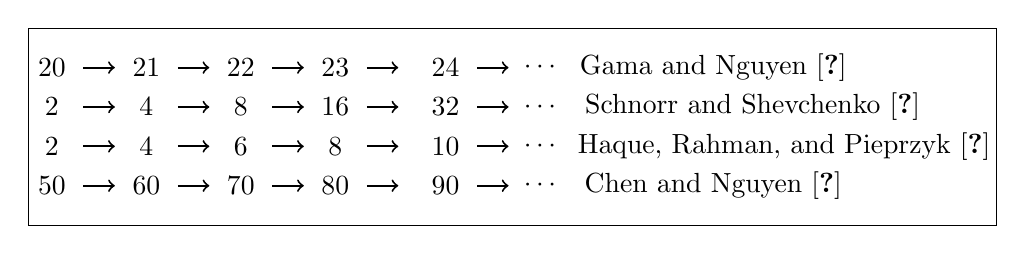
\begin{tikzpicture}
        %box drawing
        \draw[color=black] (-6.3,0) -- (6,0) -- (6,-2.5) -- (-6.3,-2.5) --  (-6.3,0);
        % horizental first
        \node at (-6,-.5) {20};
        \draw[->, line width=.25mm,  black] (-5.6,-.5)--(-5.2,-.5);
        \node at (-4.8,-.5) {21};
        \draw[->, line width=.25mm,  black] (-4.4,-.5)--(-4,-.5);
        \node at (-3.6,-.5) {22};
        \draw[->, line width=.25mm,  black] (-3.2,-.5)--(-2.8,-.5);
        \node at (-2.4,-.5) {23};
        \draw[->, line width=.25mm,  black] (-2,-.5)--(-1.6,-.5);
        \node at (-1,-.5) {24};
        \draw[->, line width=.25mm,  black] (-.6,-.5)--(-.2,-.5);
        \node at (.2,-.5) {$\cdots$};
        \node at (2.4,-.5) {\text{Gama and Nguyen} \cite{gama2008predicting}};
        % horizental Second
        \node at (-6,-1) {2};
        \draw[->, line width=.25mm,  black] (-5.6,-1)--(-5.2,-1);
        \node at (-4.8,-1) {4};
        \draw[->, line width=.25mm,  black] (-4.4,-1)--(-4,-1);
        \node at (-3.6,-1) {8};
        \draw[->, line width=.25mm,  black] (-3.2,-1)--(-2.8,-1);
        \node at (-2.4,-1) {16};
        \draw[->, line width=.25mm,  black] (-2,-1)--(-1.6,-1);
        \node at (-1,-1) {32};
        \draw[->, line width=.25mm,  black] (-.6,-1)--(-.2,-1);
        \node at (.2,-1) {$\cdots$};
        \node at (2.9,-1) {\text{Schnorr and Shevchenko} \cite{schnorr2012solving}};
        % horizental third
        \node at (-6,-1.5) {2};
        \draw[->, line width=.25mm,  black] (-5.6,-1.5)--(-5.2,-1.5);
        \node at (-4.8,-1.5) {4};
        \draw[->, line width=.25mm,  black] (-4.4,-1.5)--(-4,-1.5);
        \node at (-3.6,-1.5) {6};
        \draw[->, line width=.25mm,  black] (-3.2,-1.5)--(-2.8,-1.5);
        \node at (-2.4,-1.5) {8};
        \draw[->, line width=.25mm,  black] (-2,-1.5)--(-1.6,-1.5);
        \node at (-1,-1.5) {10};
        \draw[->, line width=.25mm,  black] (-.6,-1.5)--(-.2,-1.5);
        \node at (.2,-1.5) {$\cdots$};
        \node at (3.3,-1.5) {\text{Haque, Rahman, and Pieprzyk} \cite{haque2019analyzing}};
        % horizental fourth
        \node at (-6,-2) {50};
        \draw[->, line width=.25mm,  black] (-5.6,-2)--(-5.2,-2);
        \node at (-4.8,-2) {60};
        \draw[->, line width=.25mm,  black] (-4.4,-2)--(-4,-2);
        \node at (-3.6,-2) {70};
        \draw[->, line width=.25mm,  black] (-3.2,-2)--(-2.8,-2);
        \node at (-2.4,-2) {80};
        \draw[->, line width=.25mm,  black] (-2,-2)--(-1.6,-2);
        \node at (-1,-2) {90};
        \draw[->, line width=.25mm,  black] (-.6,-2)--(-.2,-2);
        \node at (.2,-2) {$\cdots$};
        \node at (2.4,-2) {\text{Chen and Nguyen} \cite{chen2011bkz}};
    \end{tikzpicture}
    \caption{Sequences of blocksizes that have been used after LLL-reduction in the previous literatures} %(Picture taken from \cite{laarhoven2012solving})}
    \label{fig:BKZ_Blocksize_increase}
\end{figure}
%--------------end lattice relation figure-----------------------



%Furthermore this work also proposed a simulator for predicting the length of the Gram-Schmidt basis obtained from the BKZ reduction and a model for estimating the computational cost of the proposed progressive BKZ by considering the efficient implementation of the local enumeration algorithm and the LLL algorithm. Later the work has been compare with that of other algorithms using instances from the Darmstadt SVP Challenge. Analytical experiments performed showed that the proposed algorithm is approximately $50$ times faster than that of the BKZ 2.0 when used for solving the SVP Challenge up to $160$ dimensions.


To decide the time to increase the block size $\beta$, progressive BKZ uses the Full Enumeration Cost (FEC)-- a concept derived from Gama-Nguyen-Regev's cost estimation [19] with a Gaussian heuristic radius and without pruning.
In previous works, the timing was often heuristic.
Thus, the authors in this work tried hard to develop a scientific formulation regarding time to increase the block size.

In progressive BKZ, the algorithm starts the BKZ algorithm with a relatively small blocksize $\beta_{start}$ and increases the blocksize to $\beta_{end}$.
To obtain a BKZ-$\beta$ reduced basis from a LLL reduced basis many blocksize strategies are considered as follows:
\begin{equation*}
    \beta_0^{goal}=LLL \xrightarrow{\beta_1^{alg}} \beta_1^{goal} \xrightarrow{\beta_2^{alg}} \beta_2^{goal} \xrightarrow{\beta_3^{alg}} \cdots \xrightarrow{\beta_D^{alg}}  \beta_D^{goal} (=\beta)
\end{equation*}

This sequence is also denoted by $\{(\beta_j^{alg},\beta_j^{goal})\}_{j=1,\cdots,D}$ and regarded it as the progressive BKZ.
This work employs full enumeration cost and Sim-FEC($n,\beta^{alg}$) to decide the block size increase condition.
Blocksize is increased when the condition  FEC($\pmb{B}$) $>$ Sim-FEC($n,\beta^{alg}$) fails and keeps on increasing until it reaches the condition FEC($\pmb{B}$) $<$ Sim-FEC($n,\beta^{goal}=\beta$), where $\beta^{alg}$ and $\beta^{goal}$ represents the intermediate blocksize and the target block size used in the progressive BKZ reduction.

The full enumeration cost for a basis $\pmb{B} = (\pmb{b}_1 , \cdots , \pmb{b}_n)$ of $n$-dimensional lattice $\Lambda$ is computed as
\begin{align*}
    \text{FEC}(\pmb{B}) & = \sum_{k=1}^n \frac{V_k(GH(\Lambda))}{\prod_{i=n-k+1}^n ||\pmb{b}_i^*||}
\end{align*}
where $||\pmb{b}_i^*||$ represents the GS-length.
Since $||\pmb{b}_1||$ is often larger than $\lambda_1(\Lambda)$, thus the search radius is set as $R_n=GH(\Lambda)$ to decrease the computational cost.
%Note that the FEC($\pmb{B}$) eventually decreases after performing several tours of the BKZ algorithm using the fixed blocksize $\beta$.


The simulator for an $n$-dimensional lattice depends only on the blocksize $\beta$ of the local block.
The simulated GS-length $(l_1 ,\cdots , l_n)$ is denoted by Sim-GS-lengths($n,\beta$).
A simulated Gaussian heuristic that is used in simulated GS-lengths$(l_1,\cdots,l_n)$ is defined as
\begin{align*}
    \text{Sim-GH}(l_1 , \cdots , l_n) & = V_n(1)^{-1/n} \prod_{j=1}^n l_j^{1/n}
\end{align*}
which is later used to compute the simulated value of the full enumeration cost as presented below
\begin{align*}
    \text{Sim-FEC}(l_1 , \cdots , l_n) & := \sum_{k=1}^n \frac{V_n(\text{Sim-GH}(l_1,\cdots,l_n))}{\prod_{i=n-k+1}^n l_i}
\end{align*}

%Furthermore the simulated enumeration cost Sim-ENUMCost$(l_1,\cdots,l_{\beta};\alpha,p)$ is defined by ENUMCost($B;\alpha,p$) for a lattice basis $\pmb{B}$ that has GS-lengths $||\pmb{b}^{*}_i||=l_i$ for $i \in [\beta]$.


Computation of simulated Gram-Schmidt lengths of $||b_i^*||$ using BKZ with blocksize $\beta$ performed in two steps.
In the first step, the initial value of $(l_1,\cdots,l_n)$ is computed.
This is done by setting $l_n=1$ and computing $l_i$ backwards using equation \ref{eq:l_i} below
\begin{equation}
    l_i = max \Big\{ \frac{\beta'}{\beta'+1} \alpha, \tau_{\beta'} \Big\} \cdot GH(l_i,\cdots,l_{i+\beta'-1}) \hspace{1.5em} where\ \beta'=min(\beta,n-i+1)
    \label{eq:l_i}
\end{equation}
Here $\alpha$ is the optimized radius parameter computed using equation \ref{eq:computing_r} above, and $\tau_{\beta'}$ is the coefficient of the modified Gaussian heuristic, where the modified Gaussian heuristic for $\tau_i$ is computed as
\begin{equation*}
    \tau_i= \frac{\lambda_1(\pi_{n-i+1}(\Lambda))}{GH(\pi_{n-i+1}(\Lambda))} = \frac{||\pmb{b}^{*}_{n-i+1}||} {V_i(1)^{-1/i} \cdot \prod_{j=n-i+1}^{n}||\pmb{b}^{*}_{j}||^{1/i}}
\end{equation*}


This is sufficient for the smaller block sizes viz., $\beta < 30$.
For simulating larger block sizes, we must modify the GS-lengths of the first and last indexes, and is done in the second step using the help of MINCost($\beta$), here MINCost($\beta$) represents the standard value of the enumeration cost of blocksize $\beta$.
For $i>n-\beta+1$, i.e., the situation where the blocksize is smaller than $\beta$ the modified GS-length is computed as
\begin{equation}
    l_i = max \Big\{ \frac{\beta'}{\beta'+1} \alpha_i, \tau_{\beta'} \Big\} \cdot GH(l_i,\cdots,l_{i+\beta'-1}) \hspace{1.5em} where\ \beta'=n-i+1
    \label{eq:l_i_small}
\end{equation}
Here $\alpha_i=(2/p_i)^{n-i+1}$.
Later for the first index's integer parameter, $b>0$ is used.
For $b=1,2,\cdots$ blocksize for index $i$ is computed as $\beta_i :=\beta+max\{(b-i+1),b-2(i-1)\}$ for $i\in \{1,\cdots,b\}$ using those blocksize GS-length is recomputed by using equation \ref{eq:l_i_small} from $i=\beta_i$ to $1$.
Further the value of Sim-ENUMCost($l_1 ,\cdots, l_{\beta+b}; \alpha, p$) is computed by selecting maximum $b$ that gives simulated enumeration cost smaller than $2 \cdot MINCost(\beta)$.

\begin{comment}
The expected number of BKZ tours in the progressive BKZ can be computed using equation \ref{eq:no_tours_bkz} below
\begin{equation}
    \#tours =(t-1)+ \frac{\text{Sim-FEC}(l_1',\cdots,l_n')-\text{Sim-FEC}(n,\beta)}{\text{Sim-FEC}(l_1',\cdots,l_n')-\text{Sim-FEC}(l_1,\cdots,l_n)}
    \label{eq:no_tours_bkz}
\end{equation}
Where the BKZ tour updates the pair $(l_i,l_{i+1})$ to $(l'_i,l'_{i+1})$ for $i=1,\cdots,n-1$ using the equation \ref{eq:l_i_update_1} and \ref{eq:l_i_update_2} below
\begin{align}
    l'_i     & = max \Big\{ \frac{\beta}{\beta+1}\alpha, \tau_{\beta} \Big\} \cdot GH(l_i,\cdots,l_{min(n,i+\beta-1)})
    \label{eq:l_i_update_1}                                                                                            \\
    l'_{i+1} & = l_{i+1} \cdot (l_i/l'_i)
    \label{eq:l_i_update_2}
\end{align}



Optimizing Blocksize Strategies: The optimal sequence that minimizes the total computing time can be given as
\begin{equation}
    \sum_{i=1}^D TimeBKZ(n,\beta_{i-1}^{goal} \xrightarrow{\beta_i^{alg}} \beta_i^{goal})
\end{equation}
\end{comment}


\begin{algorithm}[h!]
\KwData{Given a lattice basis $\pmb{B}$ of $n$-dimensions, Blocksize strategy $\{(\beta^{alg}_{j},\beta^{goal}_{j})\}_{j=1,\cdots,D}$}
\KwResult{A $\beta_D^{goal}$-reduced basis $\pmb{B}$}
$\pmb{B} \leftarrow LLL(\pmb{B})$; \\
\For{$j=1$ \KwTo $D$}
{
    \While{FEC($B$) $>$ Sim-FEC($n,\beta_j^{alg}$)}
    {
        \For{$i \leftarrow 1$ \KwTo $n-1$}
        {
            %Set $(\alpha,p)$ for local block $\pmb{B}_i$ of blocksize $\beta^{'}=min(\beta,n-i+1)$ \\
            %Preprocess the basis by the progressive BKZ; \\
            %Execute lattice enumeration with probability $p$ and radius $\alpha \cdot GH(\pmb{B}_i)$; \\

          %%%%%%%%%%%
          Compute the Gram-Schmidt lengths $||b^{*}_i||$ and coefficients $\mu_{ij}$ corresponding to the local block $B_i$ of blocksize $\beta'= min(\beta, n-i+1)$\\
          Set $(\alpha, p)$ for $B_i$; \\
          Set near optimized pruning coefficients $(R_1,\cdot, R_{\beta})$ for $(B_i,\alpha, p)$;
          Preprocess $B_i$ by the BKZ; \\
          \If {enumeration cost for $B_i$ computed using $(\alpha_p, R_1, \cdots , R_{\beta})$ is large}
            {
                optimize the bounding function;\\
            }
          $\{v_1, \cdots , v_h\} \leftarrow$ (lattice enumeration for $B_i$ using $(\alpha_p, R_1, \cdots , R_{\beta})$); \\
          Construct the degenerated basis \\
            $(\pmb{b}_1, \cdots , \pmb{b}_{i-1}, v_{i_1}, \cdots , v_{i_g}, b_i, \cdots , b_{i+\beta'-1})$\\
          Apply the LLL algorithm to the basis \\
            $(\pmb{b}_1, \cdots , \pmb{b}_{i-1}, \pmb{v}_{i_1}, \cdots , \pmb{v}_{i_g}, \pmb{b}_i, \cdots , \pmb{b}_{i+\beta'-1})$ \\
          and erase the zero vectors;\\
            \If {$||\pmb{v}|| < \alpha \cdot GH(\pmb{B}_i)$}
            {
                 update basis $\pmb{B}$ by $\pmb{v}$;
            }
        }
    }
}
\caption{Progressive BKZ algorithm}
\label{alg:Prog_BKZ_algo}
\end{algorithm}












\subsection{$\delta$ estimates}
In literature, few $\delta$ (root Hermite factor) estimates available for  BKZ with block size $\beta$.
These estimates can be used to predict the values of $\delta$ and/or to estimate the condition under which uSVP can be solved using lattice reduction.
We presented these estimates below:

\subsubsection{Chen estimate} Chen et al.
in \cite{chen2013reduction} estimated about $\delta$ obtained using BKZ with blocksize $\beta$ as
\begin{equation*}
    \delta(\beta)=\Big( \frac{\beta}{2\pi e} (\pi \beta)^{1/\beta} \Big) ^{\frac{1}{2(\beta-1)}}
\end{equation*}
For a large $\beta$, it is also estimated as equal to $\beta^{\frac{1}{2\beta}}$
\subsubsection{2008 estimate} Estimate provided by Gama and Nguyen in \cite{gama2008predicting} is also known as 2008 prediction.
The estimate claims that the shortest vector of a lattice can be recovered if
\begin{equation*}
    \gamma = \frac{\lambda_2}{\lambda_1} \geq \delta^n
\end{equation*}

\subsubsection{2016 estimate} Estimates provided by Alkim et al.
\cite{alkim2016post} is popularly known as the 2016 prediction.
Assuming that \textbf{Geometric Series Assumption} \cite{schnorr2003lattice} holds, the authors claimed that the norms of the Gram-Schmidt vectors after lattice reduction satisfy
\begin{equation*}
    ||\pmb{b}_i^*|| \approx \delta^{n-2i+2} \cdot Vol(\Lambda)^{1/n}
\end{equation*}
The reason behind the same is that if the projection of the unique shortest vector onto the space spanned by the last $\beta$ Gram-Schmidt vectors is shorter than $\pmb{b}_{n-\beta+1}^*$, then the SVP oracle in BKZ would be able to find it when called on the last block of size $\beta$.
Thus the success condition can be given as
\begin{equation*}
    \sqrt{\frac{\beta}{n}}\lambda_1 \leq ||\pmb{b}_{n-\beta+1}^*||
\end{equation*}



%Runtime estimates for the BKZ algorithm Dana paper as well

%Go through the new hope paper
%https://sites.math.washington.edu/~rothvoss/lecturenotes/IntOpt-and-Lattices.pdf
%https://www.youtube.com/watch?v=_WlMG81ifQs&ab_channel=TheIACR
%https://www.youtube.com/watch?v=7-RWAU8pBqI&ab_channel=TheIACR


%Runtime estimates for the BKZ algorithm Dana paper as well

%Go through the new hope paper
%https://sites.math.washington.edu/~rothvoss/lecturenotes/IntOpt-and-Lattices.pdf
%https://www.youtube.com/watch?v=_WlMG81ifQs&ab_channel=TheIACR
%https://www.youtube.com/watch?v=7-RWAU8pBqI&ab_channel=TheIACR



\subsubsection{Micciancio and Walter Prediction} In 2016, Micciancio et al.
\cite{micciancio2016practical} presented a technique to predict the output of the lattice basis reduction combining the best of both the world viz., BKZ \cite{schnorr1987hierarchy,schnorr1994lattice,chen2011bkz} and the Slide reduction algorithm introduced by Gama and Nguyen\cite{gama2008finding}.
BKZ performs well in practice; however, its asymptotic performance could be better.
Furthermore, its simple average case prediction is performed by a simulator which, in general, is based on some heuristics which need to be clarified if these hold.
Slide reduction, on the other hand, provides good simple average case prediction and asymptotic performance, but practical performance is believed to be not so great \cite{gama2008finding,gama2008predicting}.
It is claimed in \cite{gama2008finding} that BKZ with block size $k=20$ produces better-reduced bases than Slide reduction with block size $k=50$.



Thus performing an extensive experiment on several lattice reduction algorithms, both novel and from the literature, the authors claimed that to predict lattice reduction simulation is superfluous and can be replaced by a closed formula using weaker assumptions.
To reach this conclusion, the authors used a novel algorithm to solve the Shortest Vector Problem (SVP) in the dual without computing the dual basis, termed Self-Dual BKZ.
The new algorithm provides the same practical performance as that of the BKZ, asymptotic performance, and simple average case prediction as that of the Slide reduction.

\begin{comment}

\begin{algorithm}[H]
    \SetAlgoLined
    \LinesNumbered
    procedure DBKZ (\pmb{B}, k, SVP$_k$)\\
    \SetKwInOut{Input}{Input}
    \Input{A lattice basis $\pmb{B} \in \mathbb{Z}^{m\times n}$, a block size k, a SVP oracle in dimension k}
    \SetKwInOut{Output}{Output}
    \Output{A k-reduced basis $\pmb{B}'$}
    \SetKwProg{Function}{function}{}{end}
    \SetKwRepeat{Do}{do}{while}
    \While{progress is made}
    {
        Working fine
    }
    \KwRet {\pmb{B}}
    \caption{Self-Dual BKZ}
\end{algorithm}
\end{comment}


Implementation of this new SVP solving technique can be easily added to the existing primal implementation with obtained efficiency the same as that of the primal algorithm.

